\section{Resultados e Discussões}

A bateria de testes sob estresse estabeleceu as métricas e limites arquiteturais do motor Apache Druid na manipulação de grandes volumes geoespaciais, conforme consolidado a seguir.

\subsection{Matriz de Capacidade e Saturação (CPU-Bound)}

A avaliação comprovou que a renderização de mapas analíticos é severamente limitada pela capacidade de processamento matemático (\textit{CPU-Bound}).

O cenário \textbf{Baseline (1.0 CPU)} sofreu colapso imediato sob acesso concorrente, atingindo $42,7\%$ de erro (\textit{Timeouts HTTP 500}), atestando a incapacidade de um único núcleo coordenar as requisições. O cenário \textbf{Balanced (1.5 CPU)} estabilizou a plataforma com $0\%$ de erro, mas encontrou saturação aos 16 usuários concorrentes, degradando a latência P95 para 35 segundos. A alocação de meia vCPU extra no cenário \textbf{Query Heavy (2.0 CPU)} duplicou a vazão e reduziu a latência P95 pela metade (17,9 segundos).

\begin{figure}[htpb]
    \centering
    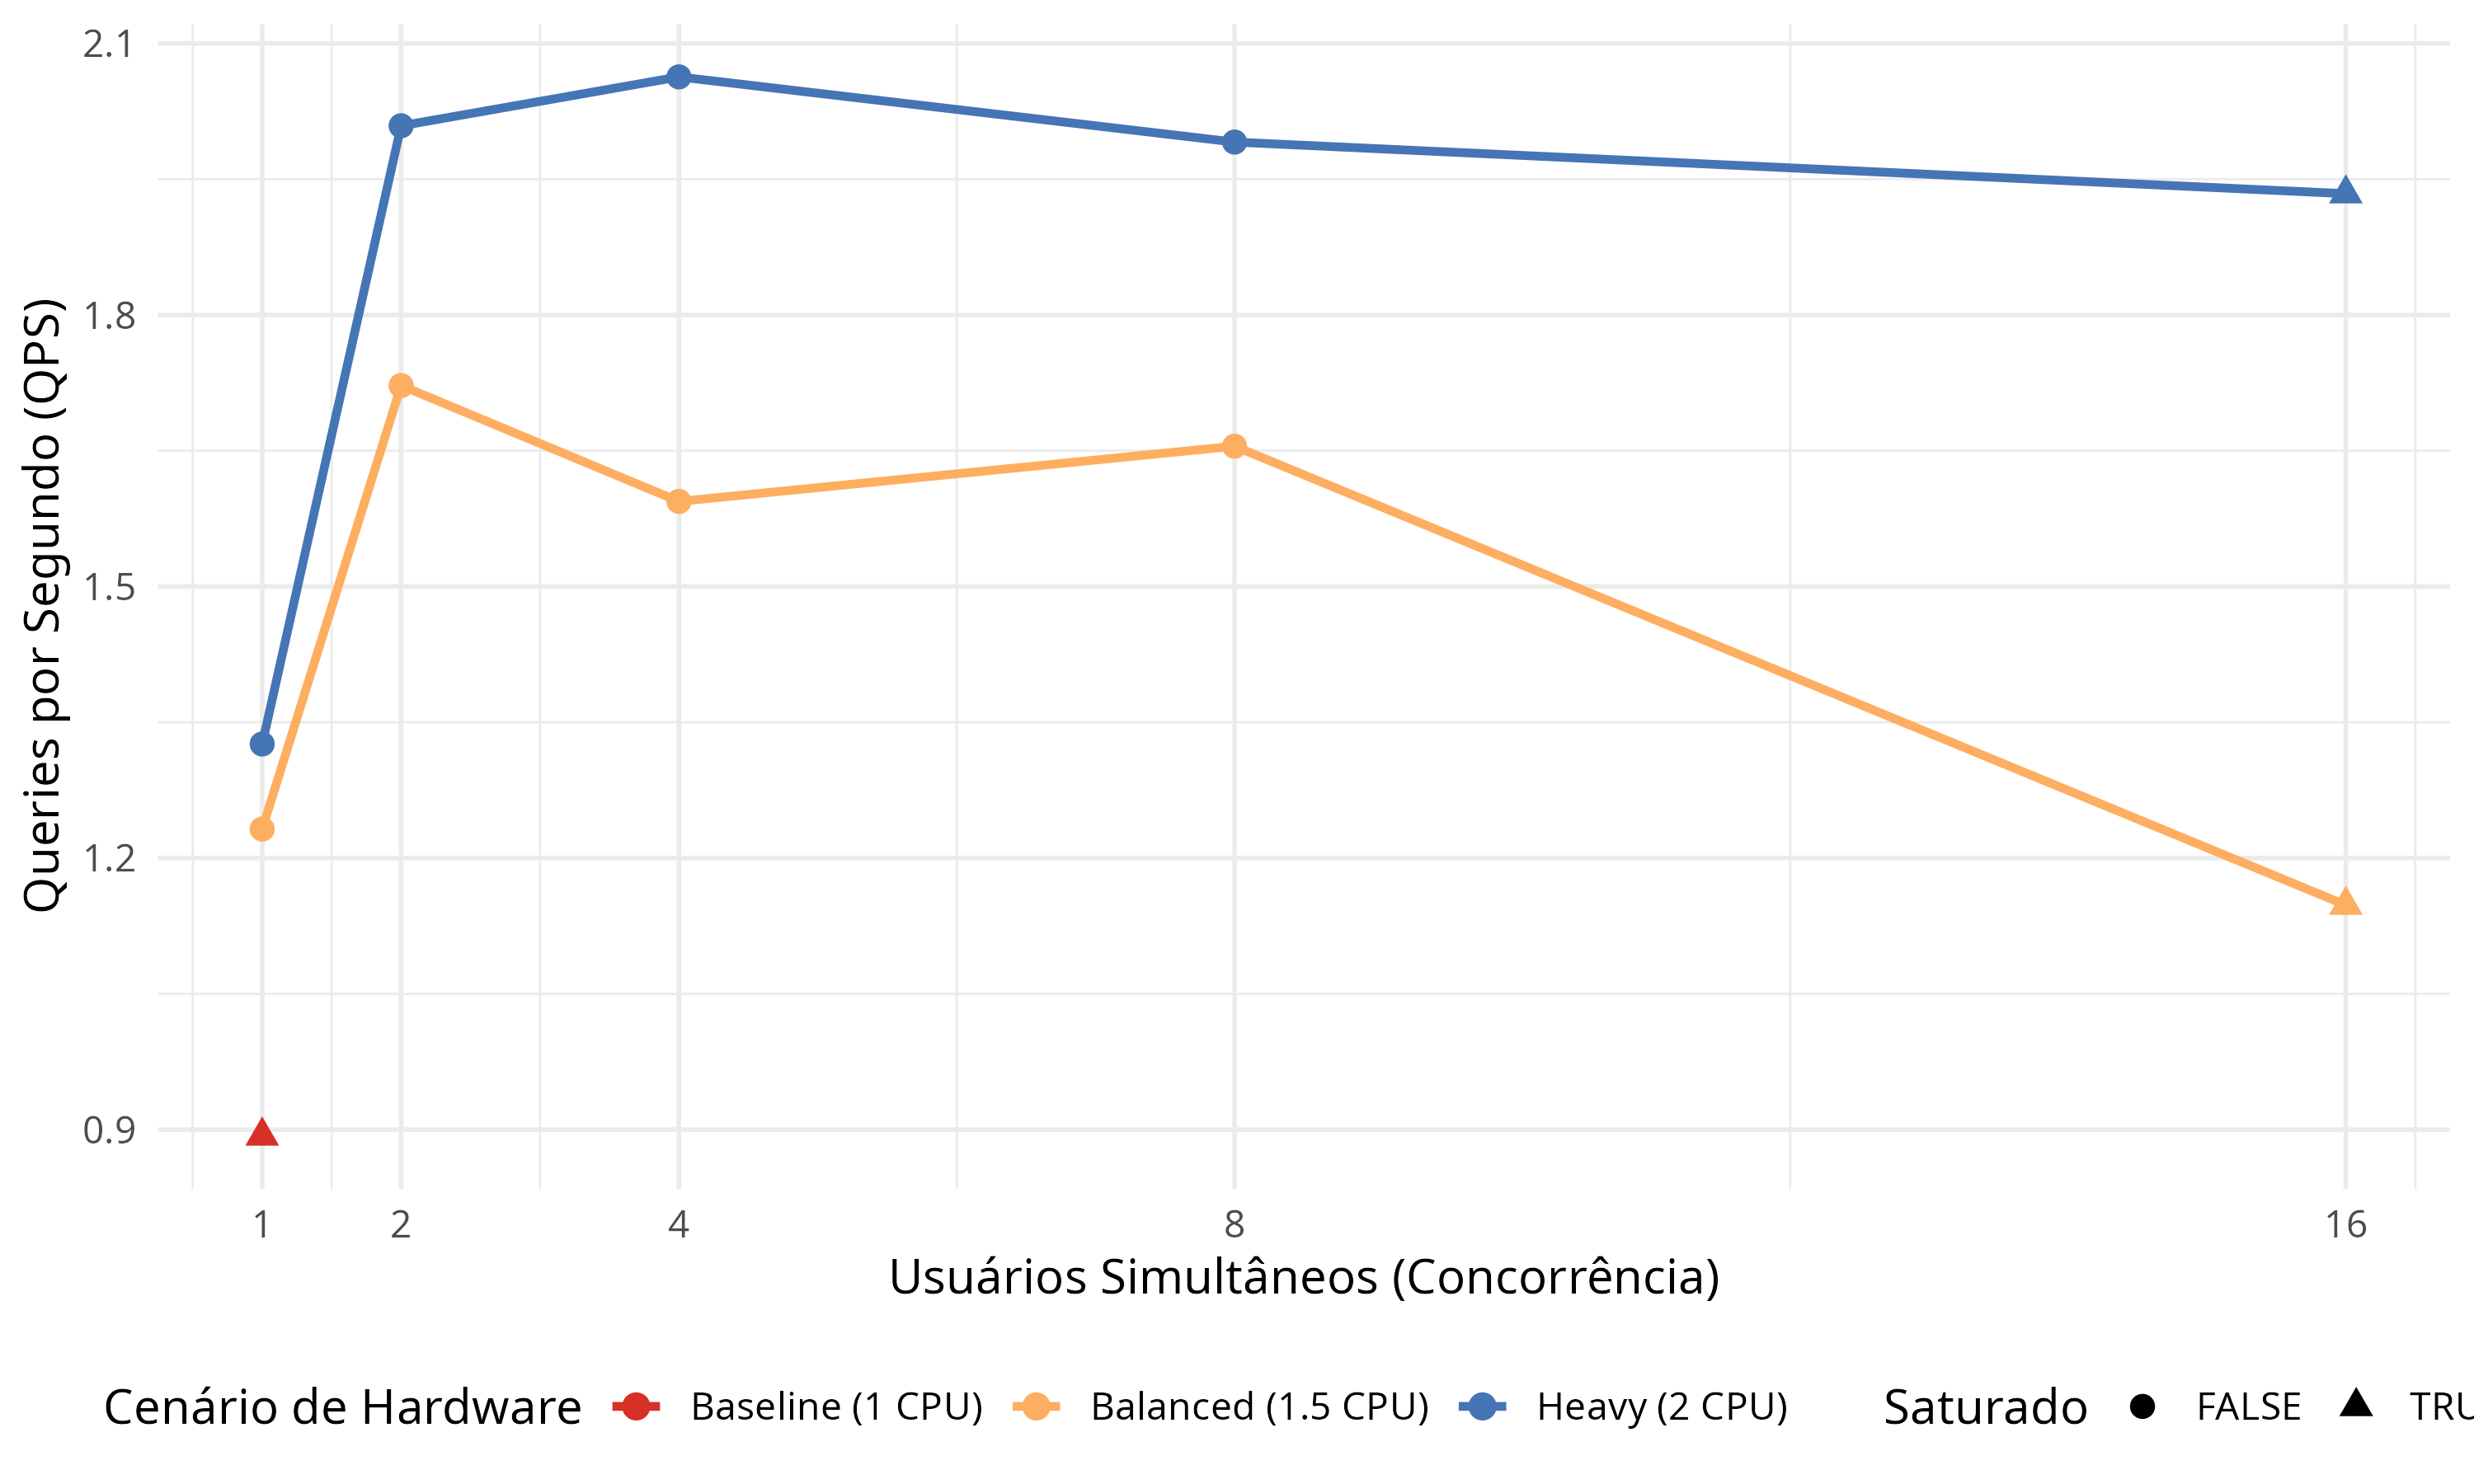
\includegraphics[width=0.8\textwidth]{images/qps_saturation.png}
    \caption{Curva de saturação: Limite de vazão da plataforma (QPS) por perfil de hardware.}
    \label{fig:qps_saturation}
\end{figure}

\begin{figure}[htpb]
    \centering
    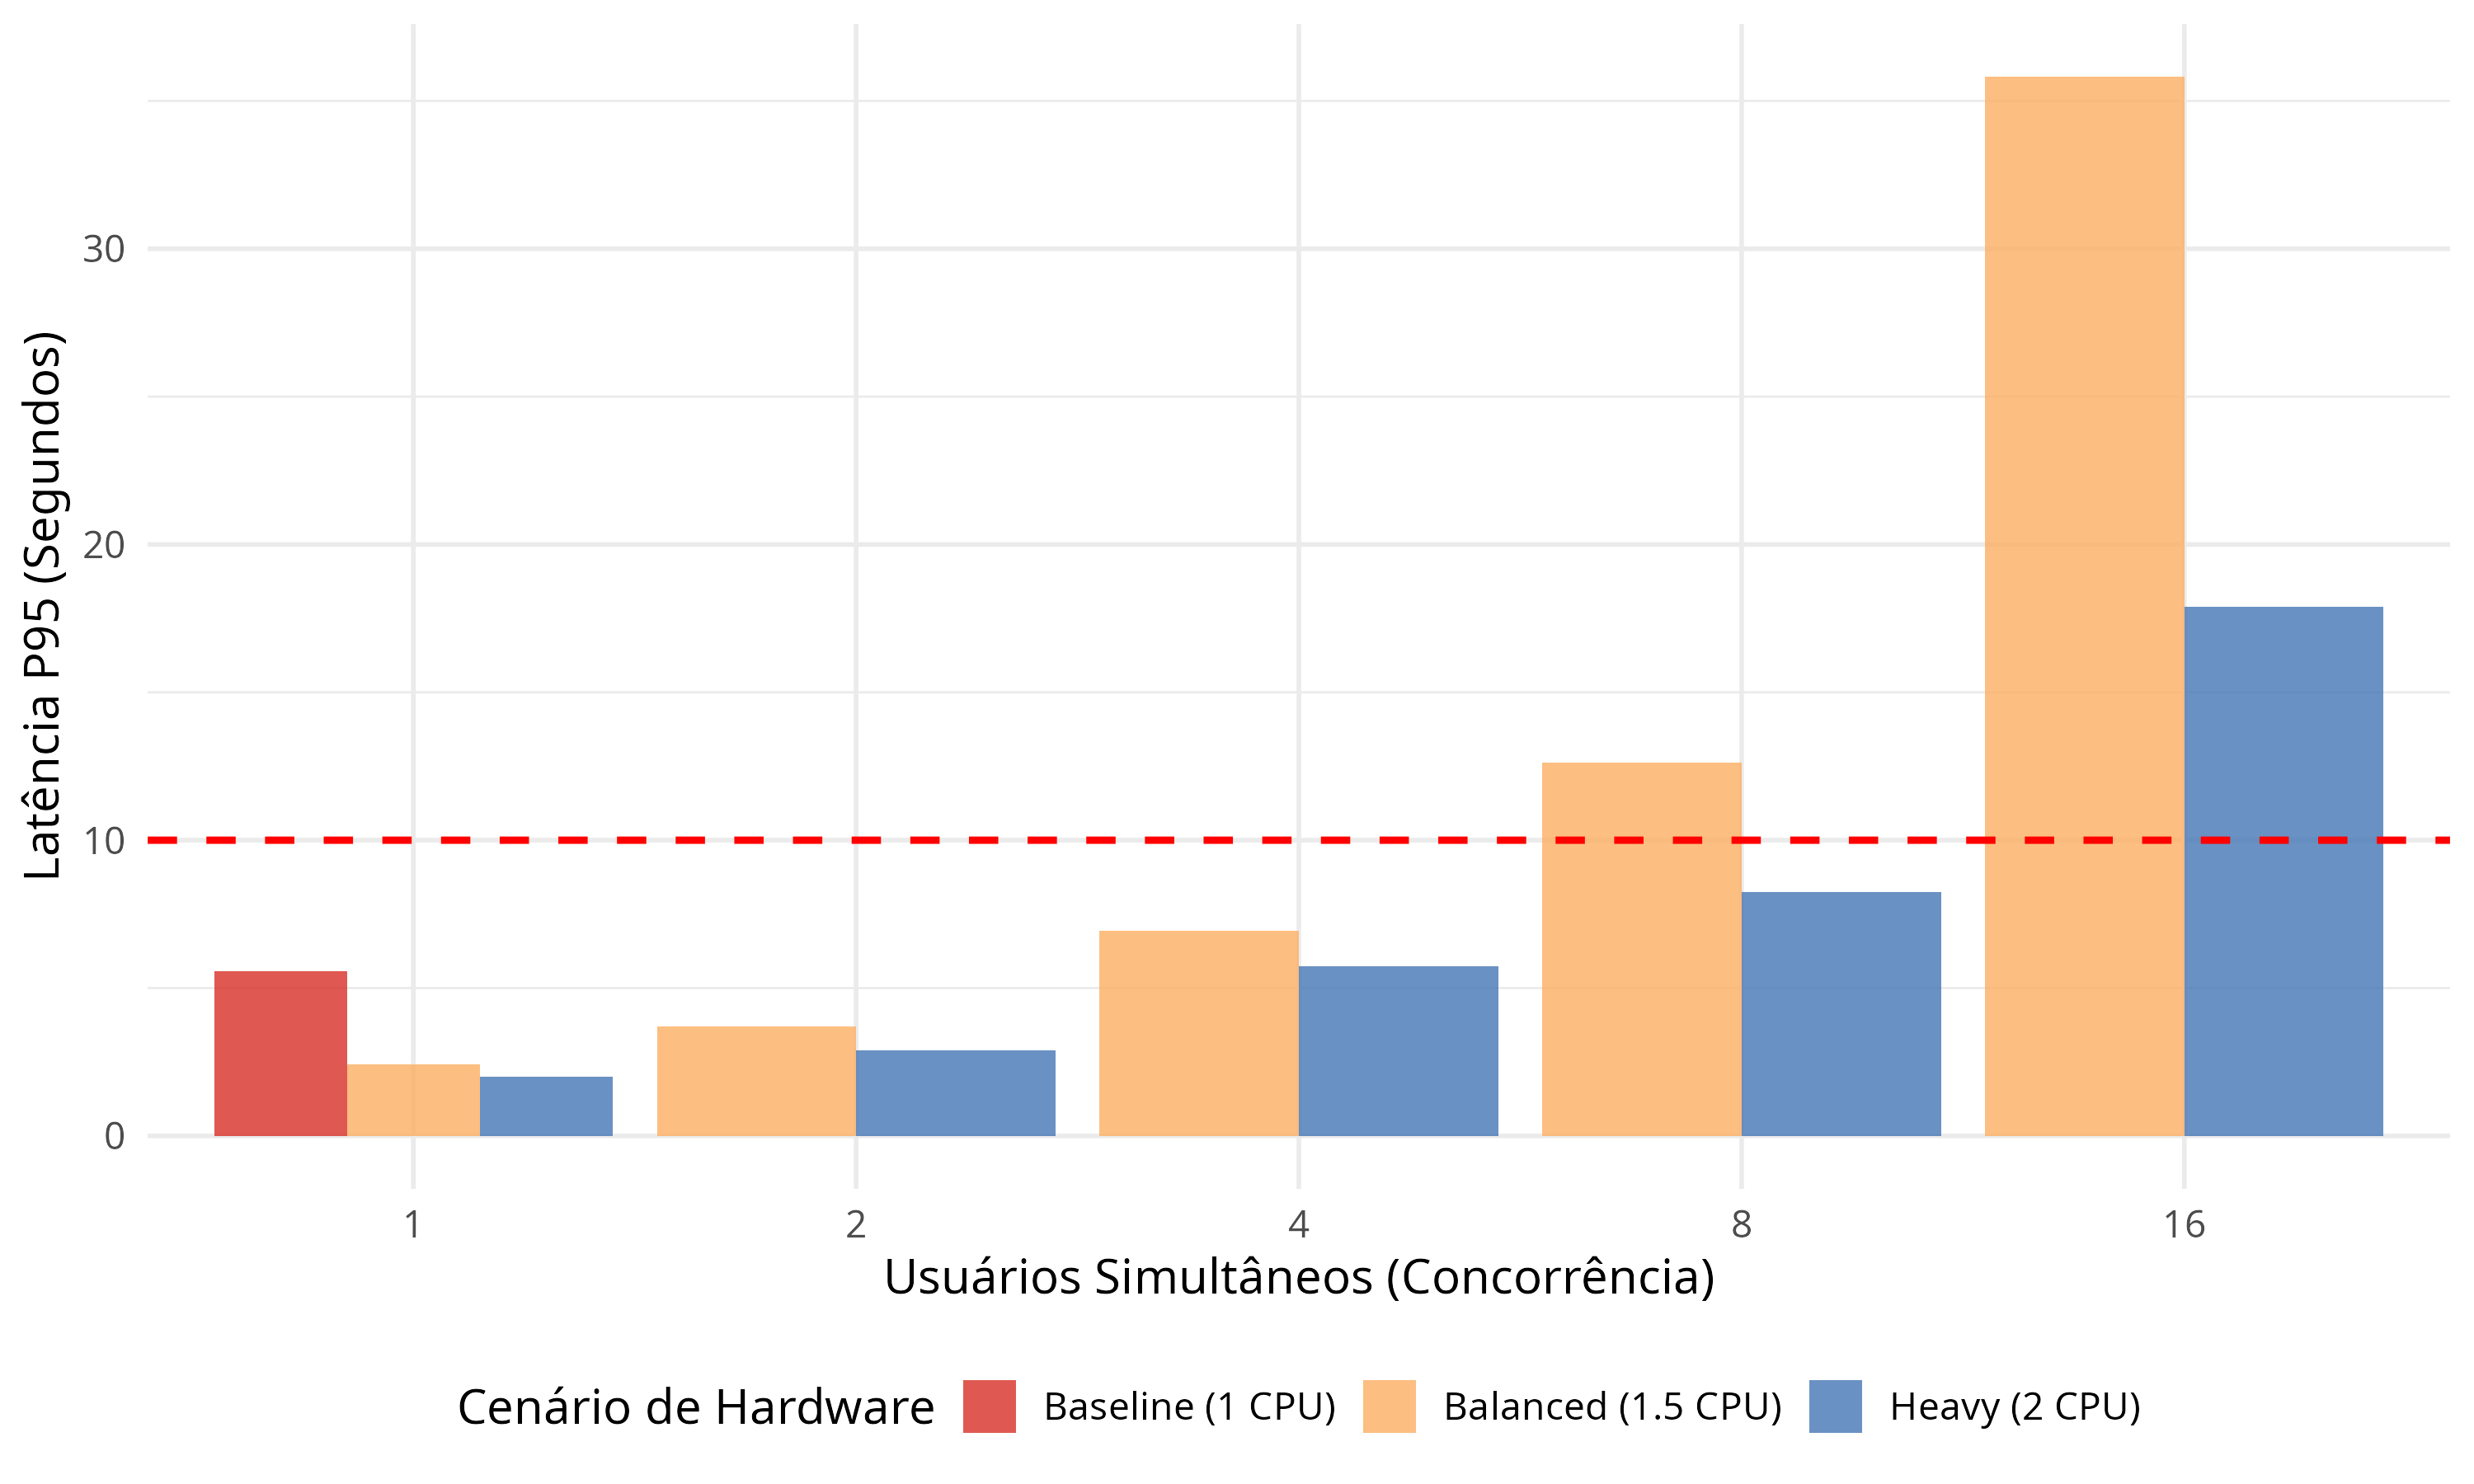
\includegraphics[width=0.8\textwidth]{images/p95_latency.png}
    \caption{Degradação da Latência P95 durante escalonamento exponencial de usuários.}
    \label{fig:p95_latency}
\end{figure}

\subsection{Eficiência do Mecanismo de Cache}

O uso do \textit{Broker Cache} no Druid acelerou varreduras completas e matrizes poligonais densas em até $40\%$. No cenário balanceado, uma extração fria (\textit{disco}) que levava $17,6s$ foi reduzida para $10,9s$ no cache (\textit{memória}). Contudo, em consultas extremamente simples (ex: \texttt{COUNT(*)} puro), o custo de rede para descriptografar a chave do cache gerou um levíssimo \textit{Overhead}, superando a velocidade da leitura nativa em colunas do disco.

\begin{figure}[htpb]
    \centering
    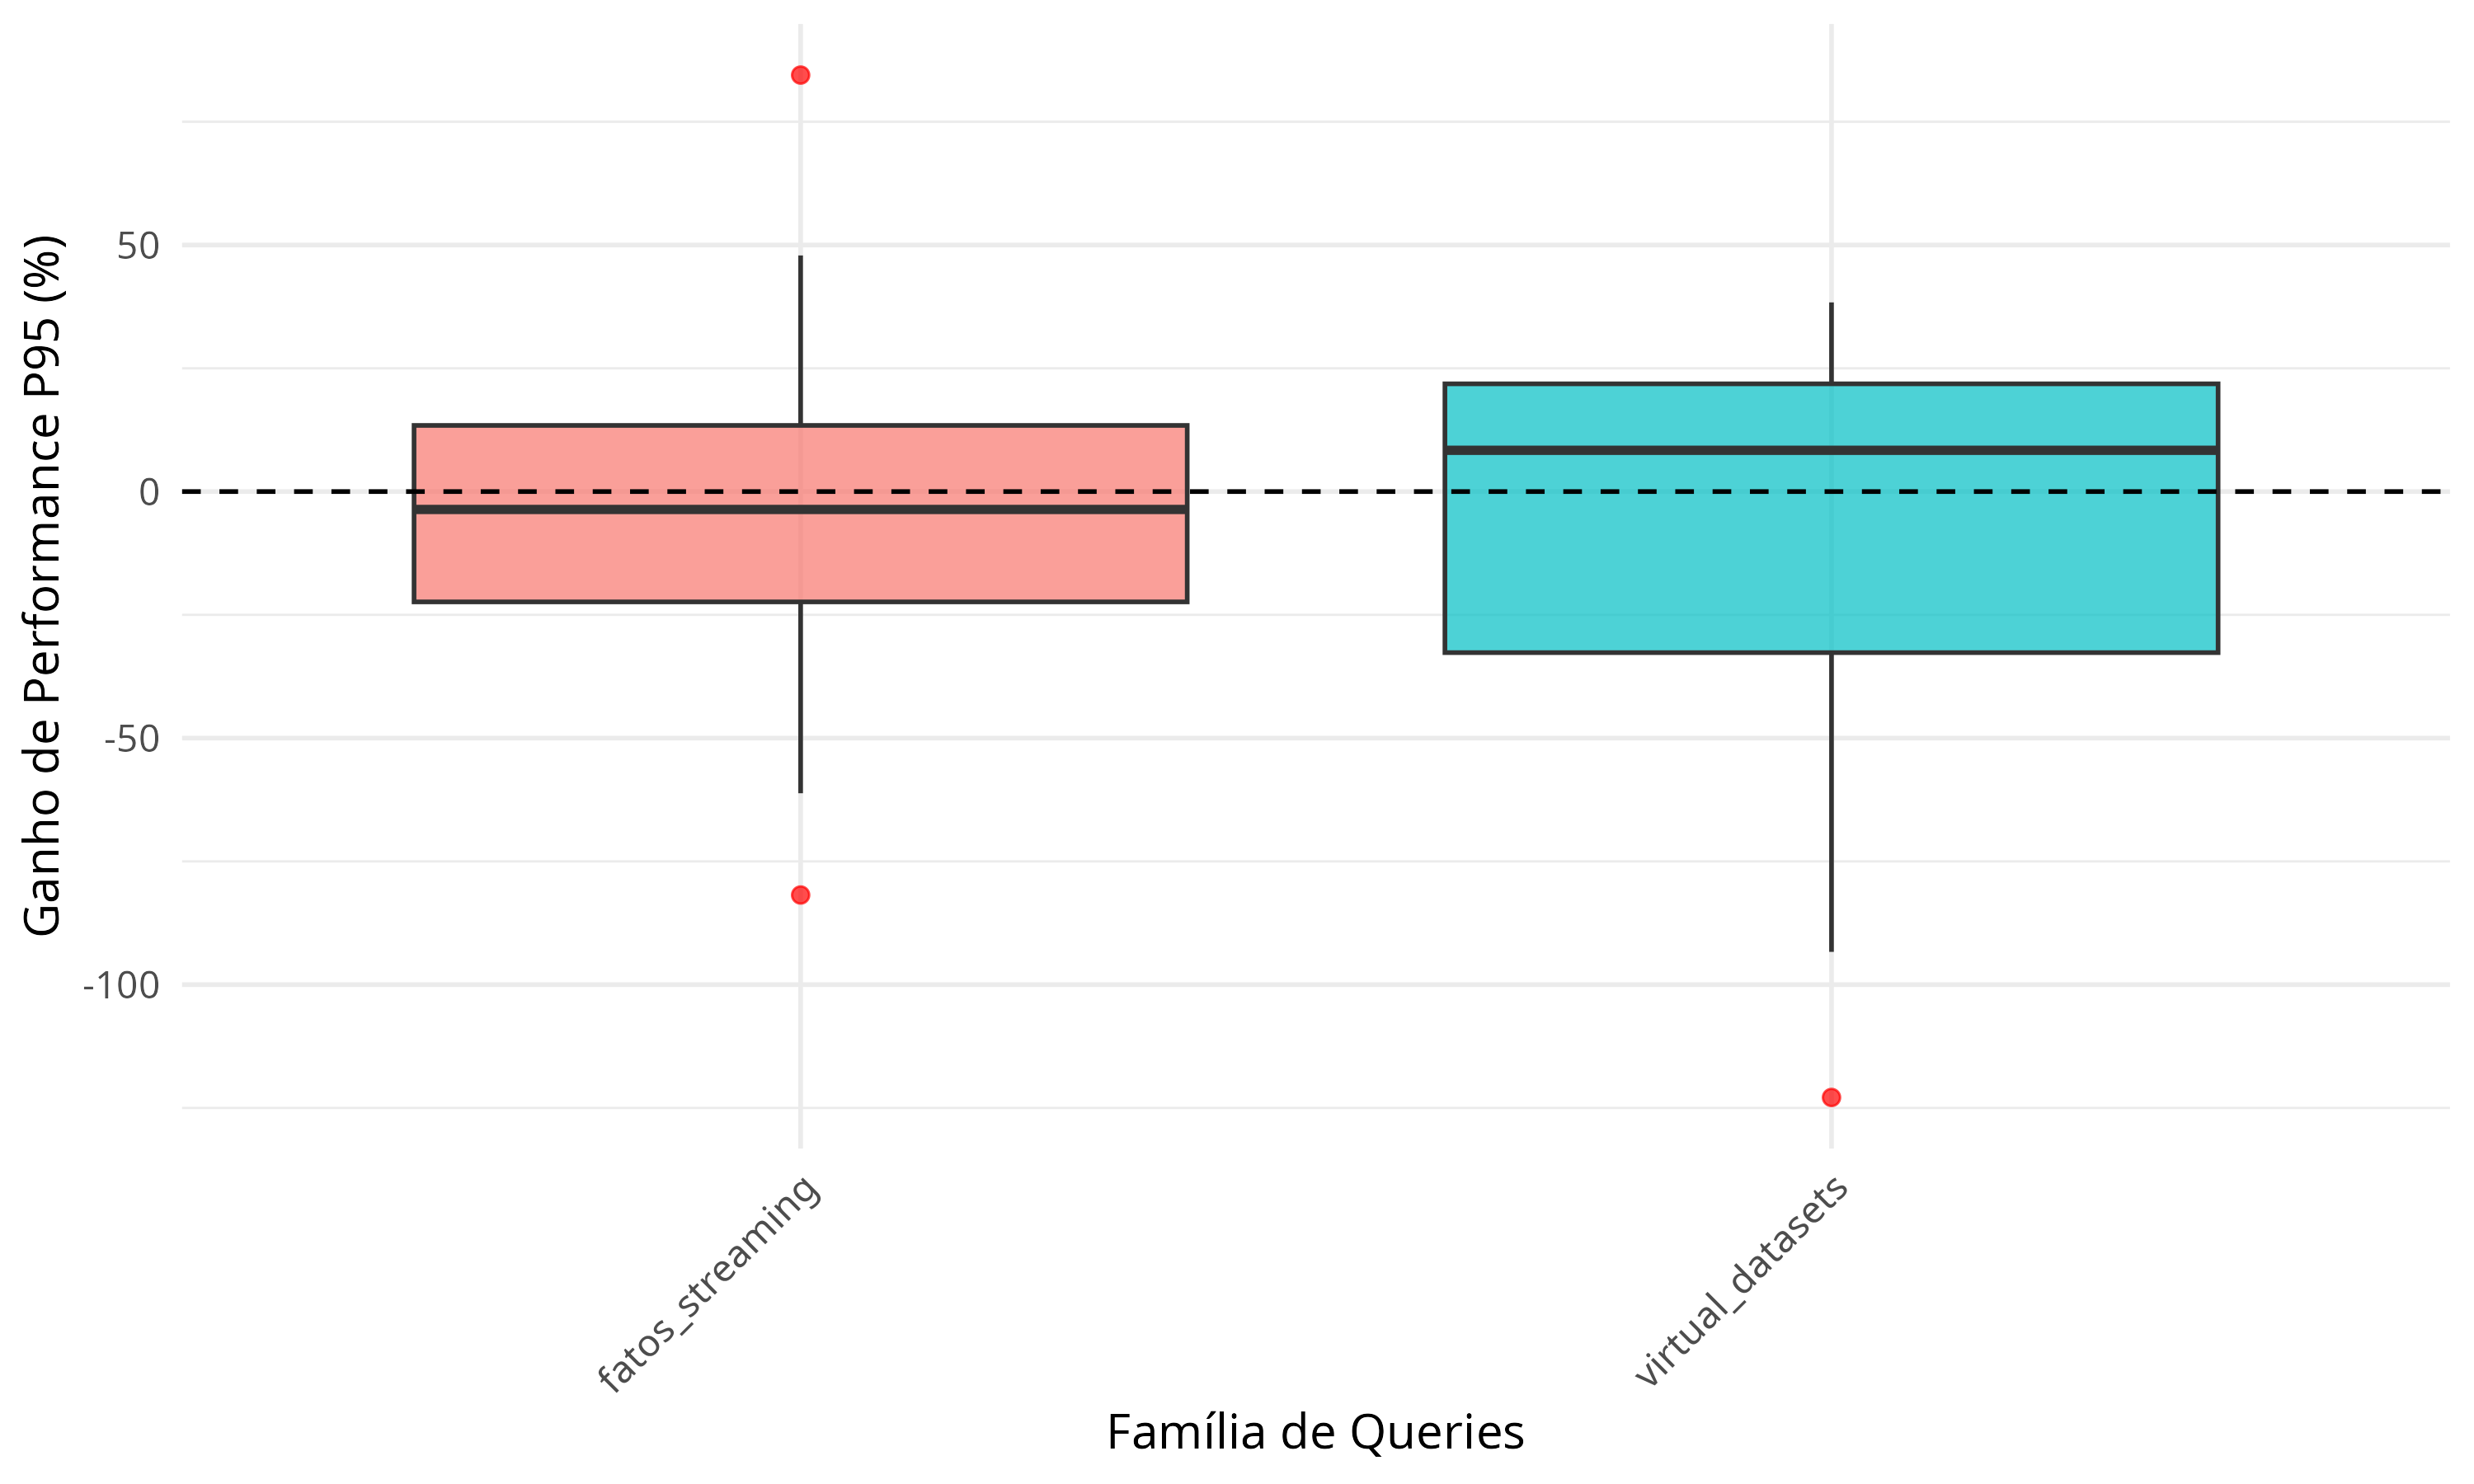
\includegraphics[width=0.8\textwidth]{images/cache_boxplot.png}
    \caption{Dispersão de ganhos obtidos entre leituras no disco (Cold) e em memória (Warm).}
    \label{fig:cache_efficiency}
\end{figure}

\subsection{Consumo Físico de Contêineres}

A análise nativa via Docker confirmou um rigoroso limite arquitetural de uso de memória. O consumo de RAM nos nós analíticos não ultrapassou $90\%$ sob as piores cargas, mantendo uma média de $75\%$. Sem episódios de troca em disco (\textit{Swap}) ou mortes lógicas (\textit{OOM Killed}), conclui-se que o gargalo restringe-se às vCPUs.

\begin{figure}[htpb]
    \centering
    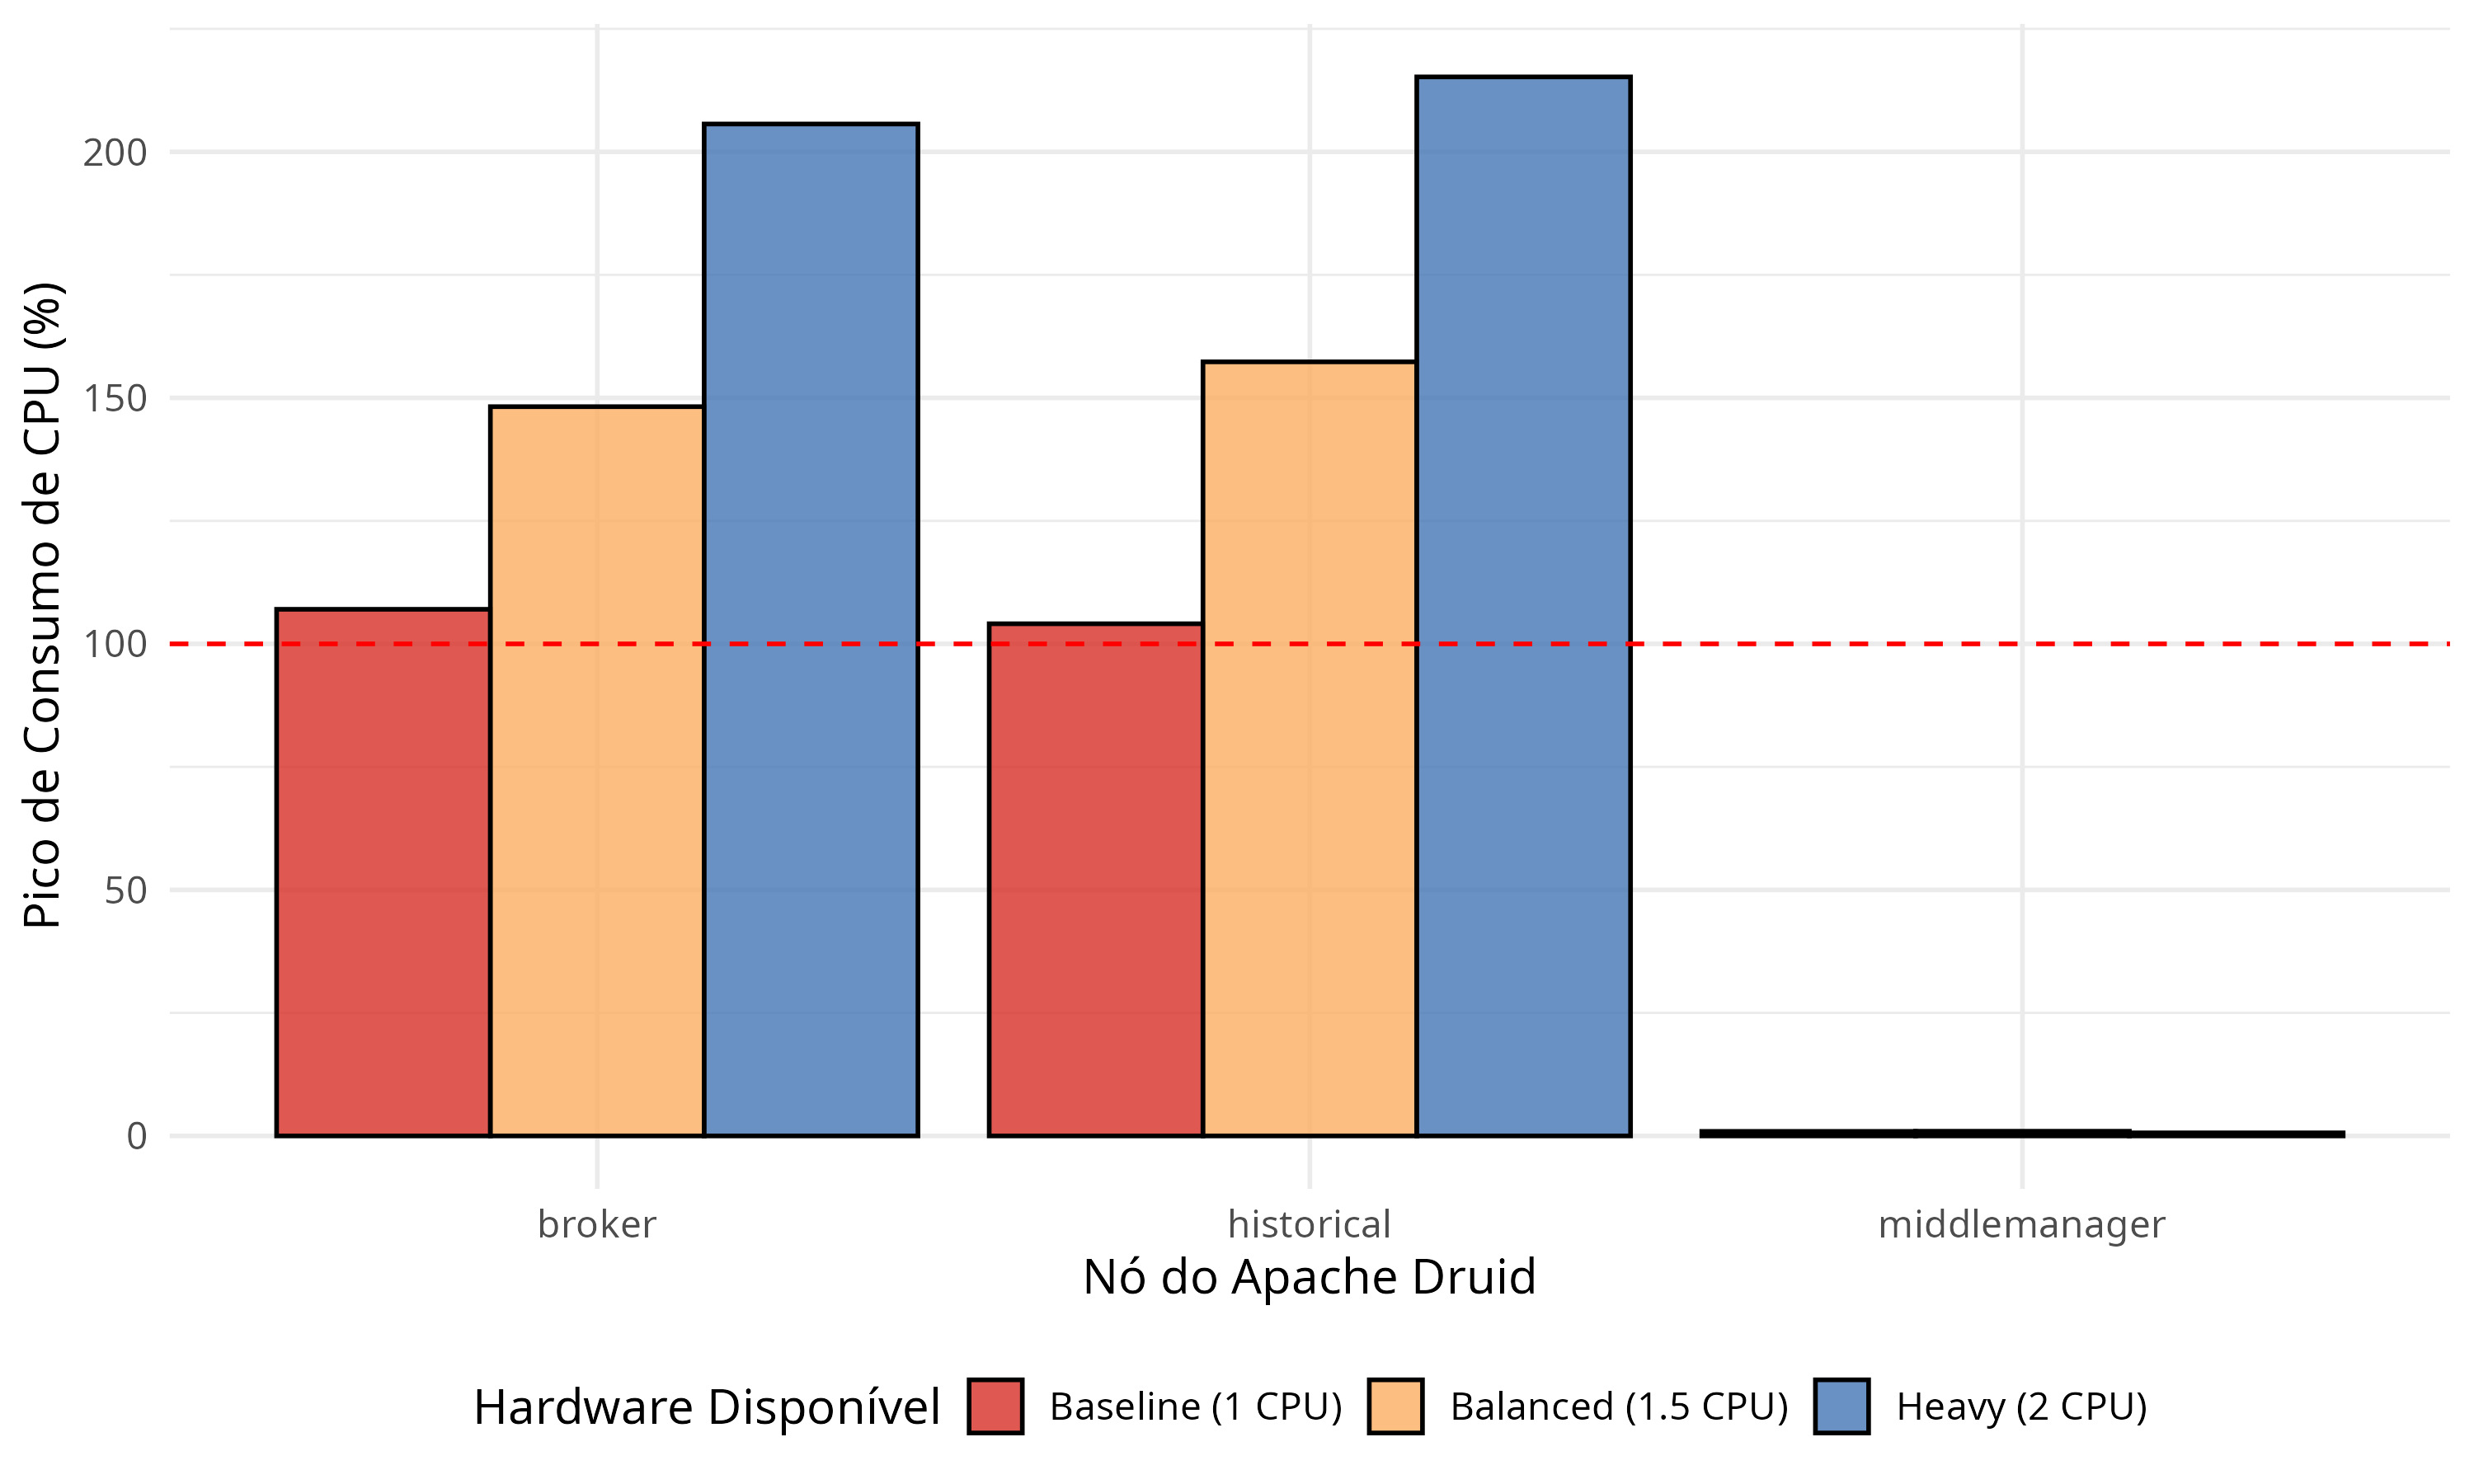
\includegraphics[width=0.8\textwidth]{images/cpu_peaks.png}
    \caption{Picos de estresse de CPU registrados por nó isolado do cluster.}
    \label{fig:cpu_peaks}
\end{figure}

\subsection{Hotspots: Gargalos Dimensionais e Armazenamento}

A consulta de maior custo foi o cruzamento espacial dinâmico, demandando longos 36 segundos sob hardware moderado. Fica provado que processar \textit{Joins} relacionais geoespaciais sob demanda limita o painel, exigindo que a desnormalização (\textit{ETL}) seja deslocada previamente para \textit{frameworks} otimizados, como o Apache Spark.

Em contrapartida à lentidão da junção analítica, a imensa vantagem do banco reflete-se na compressão extrema dos dados armazenados (Tabela~\ref{tab:storage_footprint}).

\begin{table}[htpb]
\centering
\caption{Pegada em disco consolidada das principais tabelas Fato e Dimensões.}
\label{tab:storage_footprint}
\begin{tabular}{lr}
\toprule
\textbf{Tabela (Datasource)} & \textbf{Tamanho Original (Druid)} \\
\midrule
Fato Focos (3.3M linhas) & 476 MB \\
Dimensões Terras Indígenas & 56 MB \\
Fato Eventos Clima & 34 MB \\
Outros Lookups & $\sim$1 MB \\
\midrule
\textbf{Total Compactado} & \textbf{566 MB} \\
\bottomrule
\end{tabular}
\end{table}
